\subsubsection*{\underline{\textsc{\Large Zombie}}}
\noindent\emph{Medium undead, neutral evil}

Undead zombies move with a jerky, uneven gait. They are clad in the moldering apparel they wore when put to rest, and carry the stench of decay.

\noindent\rule{0.5\textwidth}{0.5pt}

\noindent\textbf{Armor Class}: 8

\noindent\textbf{Hit Points}: 22 (3d8 + 9)

\noindent\textbf{Speed}: 20 ft.

\noindent\rule{0.5\textwidth}{0.5pt} \\
\begin{table}[H]
	\begin{tabular}{cccccc}
		\textbf{STR} & \textbf{DEX} & \textbf{CON} & \textbf{INT} & \textbf{WIS} & \textbf{CHA} \\
		13 (+1) & 6 (-2) & 16 (+3) & 3 (-4) & 6 (-2) & 5 (-3) \\
	\end{tabular}
\end{table}
\noindent\rule{0.5\textwidth}{0.5pt} \\

\noindent\textbf{Saving Throws}: Wis +0

\noindent\textbf{Damage Immunities}: poison

\noindent\textbf{Condition Immunities}: poisoned

\noindent\textbf{Senses}: darkvision 60 ft., passive Perception 8

\noindent\textbf{Languages}: understands the languages it knew in life but can't speak

\noindent\textbf{Challenge}: 1/4 (50 XP)

\noindent\rule{0.5\textwidth}{0.5pt}

\noindent\textbf{Undead Fortitude}: If damage reduces the zombie to 0 hit points, it must make a Constitution saving throw with a DC of 5 + the damage taken, unless the damage is radiant or from a critical hit. On a success, the zombie drops to 1 hit point instead.

\noindent\rule{0.5\textwidth}{0.5pt}

\noindent\textbf{ACTIONS}

\noindent\textbf{Slam}: Melee Weapon Attack: +3 to hit, reach 5 ft., one target. Hit: 4 (1d6 + 1) bludgeoning damage.

\begin{center}
	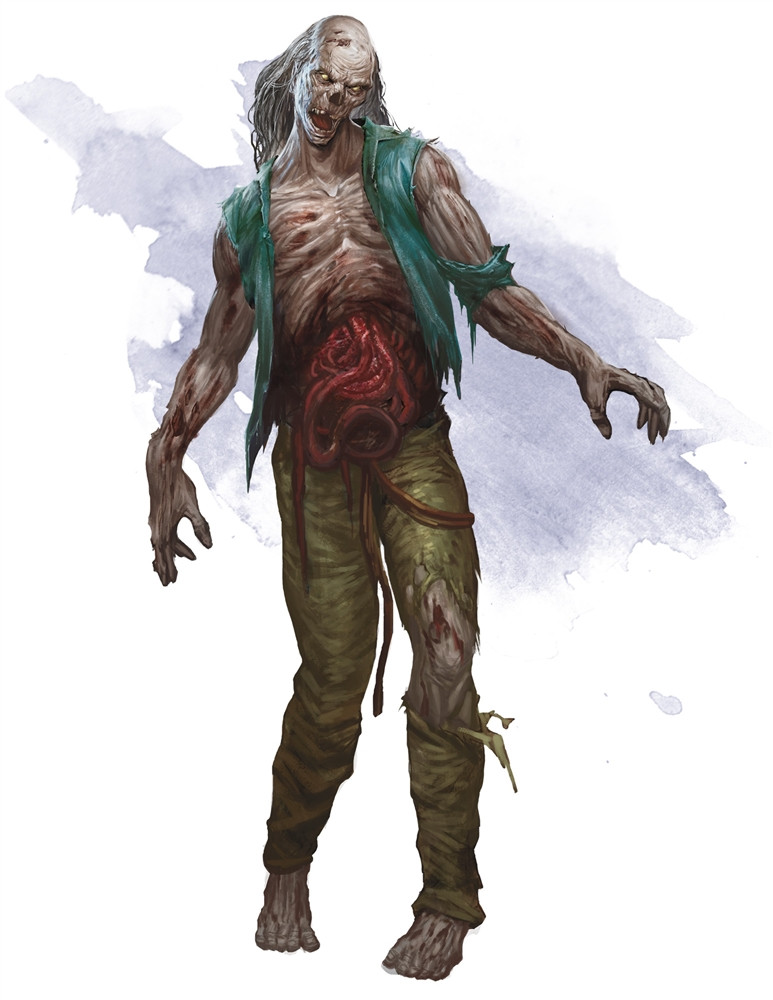
\includegraphics[width = 0.3\textwidth]{zombie}
	
	\emph{Zombie}
\end{center}